\section{Auswertung}
\subsection{Vorbereitung}
In der vorbereitenden Aufgabe wird zunächst die Flussdichte $B_0$ für einen Strom I von 1A berechnet. Hierfür wird [FORMEL] verwendet
sowie die Werte für das Helmholtz-Spulenpaar, welche in Kapitel [KAPITEL] zu finden sind.
Wird für die magnetische Feldkonstante $\mu_0 = 1.26 \cdot 10^{-6} \symup{\frac{N}{A^2}}$ verwendet, ergibt sich eine Flussdichte
von 
\begin{equation*}
B_0 = 4.86\cdot 10^{-3} \symup{T}.
\end{equation*}

Weiterhin wird mit [FORMEL] das Trägheitsmoment $J_{\text{K}}$ der im Versuch verwendeten Billiardkugel mit 
\begin{equation*}
\begin{aligned}
r_{\text{K}} &= 2.5\symup{cm}, \\
m_{\text{K}} &= 150\symup{g}
\end{aligned}
\end{equation*}
ermittelt. Das Trägheitsmoment beträgt damit $J_{\text{K}} = 3,75 \cdot 10^{-5} \symup{kg m^2}$.

%-----------------------------------------------------

\subsection{Bestimmung des magnetischen Momentes unter Ausnutzung der Gravitation}
Die in dieser Methode eingestellten Ströme und gemessenen Abstände r sind in Tabelle \eqref{tab:tabellegravmethode} zu finden. Die zu 
den Strömen gehörigen Flussdichten B können mithilfe der Vorbereitungsaufgabe ermittelt werden, indem $B_0$ jeweils mit den 
verschiedenen Strömen multipliziert wird.

\begin{table}[htbp]
\centering
\caption{Gravitationsmethode: Ermittelte Größen}
\label{tab:tabellegravmethode}
\begin{tabular}{S[table-format=1.1] S[table-format=2.2] S[table-format=1.1]}
\toprule
 {$I/\symup{A}$} & {$B/10^{-3}\symup{T}$} & {$r/10^{-2}\symup{m}$} \\
\midrule
2.0 &  9.72 & 2.7 \\
2.3 & 11.18 & 3.5 \\
2.5 & 12.15 & 4.7 \\
2.6 & 12.64 & 4.5 \\
2.8 & 13.61 & 5.9 \\
3.0 & 14.58 & 4.2 \\
3.2 & 15.55 & 7.6 \\
3.5 & 17.01 & 7.3 \\
3.7 & 17.98 & 8.8 \\
4.0 & 19.44 & 9.3 \\

\bottomrule
\end{tabular}
\end{table}

Es wird nun r gegen B aufgetragen, wie in Abbildung \eqref{fig:bildgravmethode} zu sehen ist.
\begin{figure}[h]
\centering
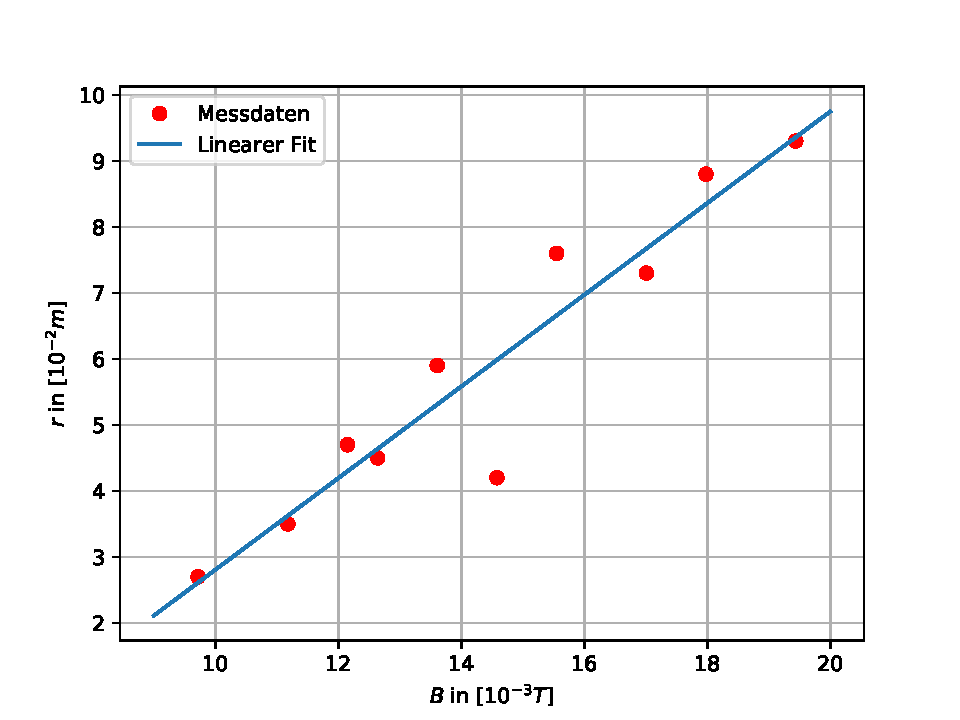
\includegraphics[scale=.9]{GravMethode.pdf}
\caption{Gravitation}
\label{fig:bildgravmethode}
\end{figure}
Die Steigung der eingezeichneten Ausgleichsgerade beträgt $\frac {r}{B}= (6.94 \pm 0.84) \symup{\frac{m}{T}}$.
Nach Umstellen von Gleichung [Mü und B/R und soo!!] lässt sich so ein magnetisches Moment von $\mu_{\text{Dipol}} = (0.0953 \pm 0.0115)
\symup{\frac{J}{T}}$ berechnen. Das Gewicht der kleinen Masse m beträgt $m = 0.0014 \symup{kg}$, die Erdbeschleunigung
ist hier $g = 9.81 \symup{\frac{m}{s^2}}$.


%-----------------------------------------------------
\subsection{Bestimmung des magnetischen Momentes über die Schwingungsdauer}
In diese Messmethode wird das magnetische Moment $\mu_{\text{Dipol}}$ über Gleichung [GLEICHUNG] ermittelt. In der Vorbereitung 
wurde das benötigte Trägheitsmoment der Billiardkugel bereits zu $J_{\text{K}} = 3.75 \cdot 10^{-5} \symup{kg m^2}$ bestimmt.
In Tabelle \eqref{tab:tabelleschwingung} sind die eingestellten Ströme sowie die gemessenen Periodendauern zu finden.
\begin{table}[htbp]
\centering
\caption{Schwingungsmethode: Ermittelte Größen}
\label{tab:tabelleschwingung}
\begin{tabular}{S[table-format=1.1] S[table-format=2.2] S[table-format=3.2] S[table-format=1.3] S[table-format=1.3]}
\toprule
 {$I/\symup{A}$} & {$B/10^{-3}\symup{T}$} & {$\frac{1}{B}/T$} & {$T/s$} & {$T^2/s^2$} \\
\midrule
2.0 &  9.72 & 102.88 & 1.172 & 1.374 \\
2.3 & 11.18 & 89.45 & 1.106 & 1.223 \\
2.5 & 12.15 & 82.30 & 1.053 & 1.109 \\
2.6 & 12.64 & 79.11 & 1.038 & 1.077 \\
2.8 & 13.61 & 73.47 & 0.991 & 0.982 \\
3.0 & 14.58 & 68.59 & 0.963 & 0.927 \\
3.2 & 15.55 & 64.31 & 0.931 & 0.867 \\
3.5 & 17.01 & 58.79 & 0.897 & 0.805 \\
3.7 & 17.98 & 55.62 & 0.860 & 0.739 \\
4.0 & 19.44 & 51.44 & 0.768 & 0.589 \\

\bottomrule
\end{tabular}
\end{table}

\begin{figure}[htbp]
\centering
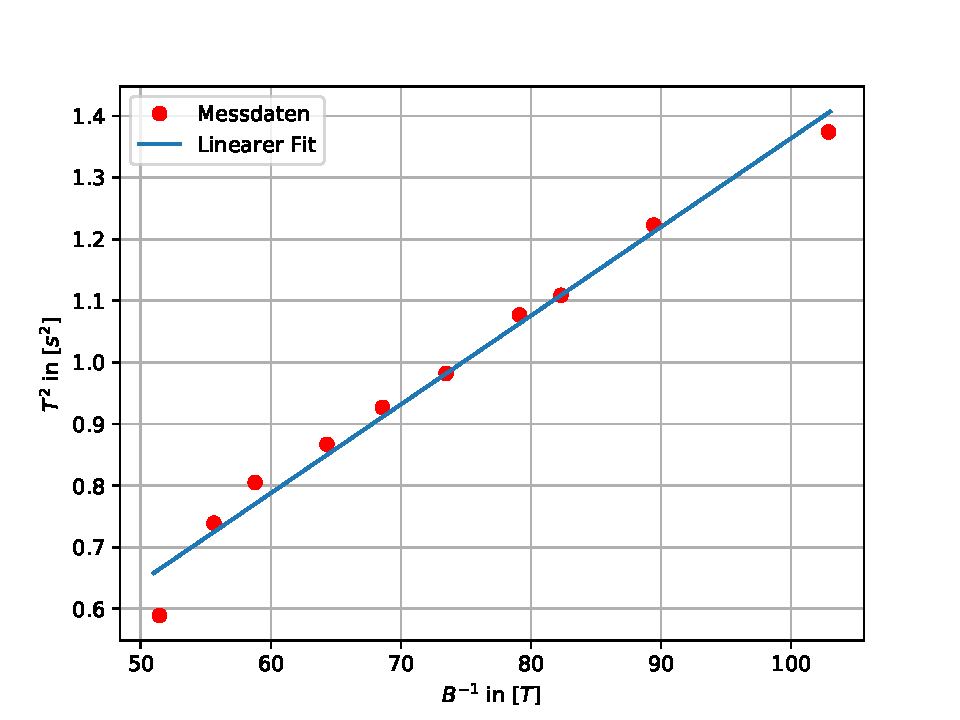
\includegraphics[scale=.9]{SchwingungsMethode.pdf}
\caption{Schwingung}
\label{fig:bildschwingung}
\end{figure}
Die Steigung der Ausgleichgeraden beträgt $T^2\cdot B = (0.0144 \pm 0.0007) \symup{s^2\cdot T}$. 
Dies kann in Gleichung  [GLEICHUNG] eingesetzt werden und erhält ein magnetisches Moment von 
$\mu_{\text{Dipol}}= (0.1027892525 \pm 2.4674 ) \symup{\frac{J}{T}}$.


%-----------------------------------------------------
\subsection{Bestimmung des magnetischen Moments über die Präzession}
Mit Gleichung [GLEICHUNG] kann $\mu_{\text{Dipol}}$ über die Präzessionsmethode berechnet werden. Der Drehimpuls $L_{\text{K}}$ ist
\begin{equation}
L_{\text{K}} = J_{\text{K}} \cdot 2\pi \nu
\end{equation}
$J_{\text{K}}$ kann aus der Vorbereitung entnommen werden, die Frequenz $\nu$ beträgt 5.8Hz. $L_{\text{K}}$ beträgt damit 
$1.367\cdot 10^{-3} \frac{kg\cdot m^2}{s}$.

Aus Tabelle \eqref{tab:tabellepraezi} können die Ströme, die daraus resultierenden magnetischen Flussdichten und die reziproken Periodendauern 
entnommen werden.
\begin{table}[htbp]
\centering
\caption{Präzessionsmethode: Ermittelte Größen}
\label{tab:tabellepraezi}
\begin{tabular}{S[table-format=1.1] S[table-format=2.2] S[table-format=2.2] S[table-format=2.2] S[table-format=2.2]}
\toprule
 {$I/\symup{A}$} & {$B/10^{-3}\symup{T}$} & {$T_1/s$} & {$T_2/s$} & {$T_3/s$} \\
\midrule
0.5 &  2.43 & 25.28 & 25.06 & 20.88 \\
1.0 &  4.86 & 12.88 & 15.15 & 15.75 \\
1.5 &  7.29 & 10.06 &  8.13 &  8.60 \\
2.0 &  9.72 &  8.31 &  8.04 &  7.50 \\
2.5 & 12.15 &  6.69 &  5.91 &  5.90 \\
2.7 & 13.12 &  6.59 &  6.69 &  7.29 \\
3.0 & 14.58 &  4.62 &  5.78 &  6.06 \\
3.5 & 17.01 &  4.66 &  5.09 &  4.59 \\
3.7 & 17.98 &  4.69 &  4.37 &  5.09 \\
4.0 & 19.44 &  5.00 &  4.81 &  4.50 \\

\bottomrule
\end{tabular}
\end{table}
\begin{figure}[h]
\centering
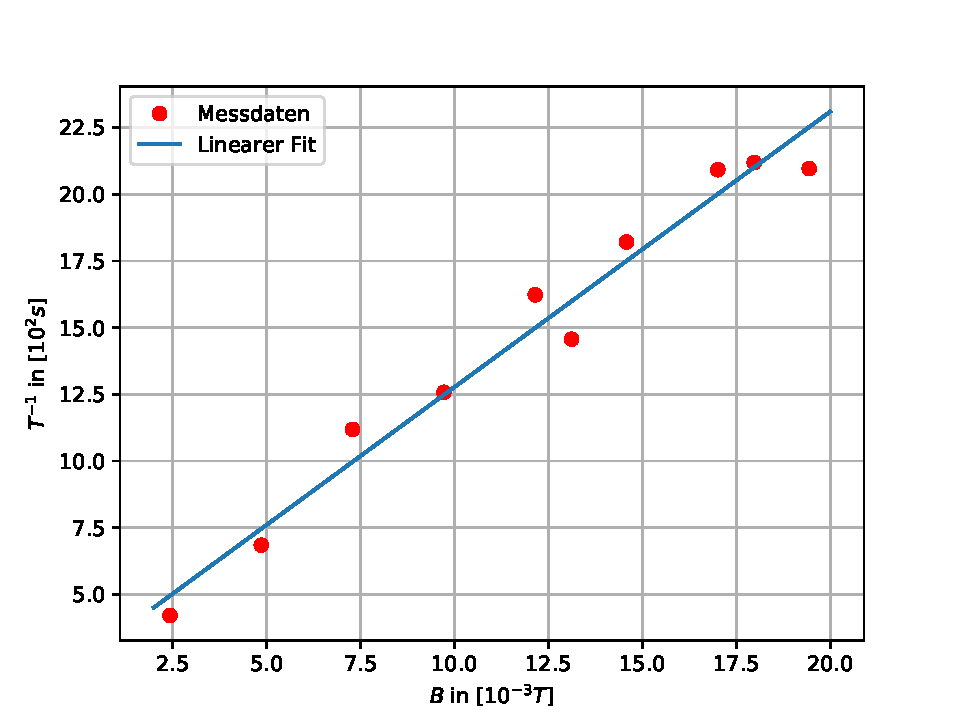
\includegraphics[scale=.9]{PraezessionsMethode.pdf}
\caption{Präzession}
\label{fig:bildpraezi}
\end{figure}
In Abbildung \eqref{fig:bildpraezi} wurden die gemittelten, reziproken Periodendauern $T_{\text{p}}$ gegen die magnetischen 
Flussdichten aufgetragen. 
Die Steigung beträgt $\frac{1}{T_{\text{p}} \cdot B} = (10.3261 \pm 0.6448) \frac{1}{s\cdot T}$. Das magnetische Moment
ist somit $\mu_{\text{Dipol}} = (0.0887 \pm 0.0054) \frac{J}{T}$.
